\fakesection{Simuleren van Sparen en Beleggen}

\begin{center}
\textit{De broncode bevindt zich in de \texttt{src} folder. Het algemene script (\texttt{src/s0216676\_script}) is opgedeeld in secties, \'e\'en per opgave. Elke opgave wordt hieronder afzonderlijk beantwoord. Aan het einde van elk antwoord wordt (indien nodig) de broncode weergegeven.}
\end{center}

%%%
%%%
%%%

\fakesubsection{Opdracht 1}

Hier is een implementatie :

\begin{lstlisting}
function [yield, invested, value] = s0216676_simulateSavingInvesting(budget, rate, months)
    value = repelem(budget * 1.02 .^ (0:floor(months/12)), 1, 12); 
    invested = sum(value(1:months));
    for j = 13:12:months % Consider each month of january
    	win = sum(value(j-12:j-1) .* (((12:-1:1)/12) * (rate/100))); % Calculate savings
    	value(j) = value(j) + (win - 0.15 * (win > 980) * (win - 980));
        value(j-12:j) = cumsum(value(j-12:j)); % Accumulate sums
    end
    value = value(1:months); value(j:end) = cumsum(value(j:end));
    yield = value(months) / invested - 1;
end
\end{lstlisting}

%%%
%%%
%%%

\fakesubsection{Opdracht 2}

Het resultaat van de gegeven code is te zien in figuur \ref{fig:op2}. De totale investering bedraagt zo'n 96091 euro. De relatieve winsten bedragen 5.46\%, 11.34\%, 23.34\% en 50.82\%.

\vspace{0.3cm}
\begin{figure}[h]
\centering
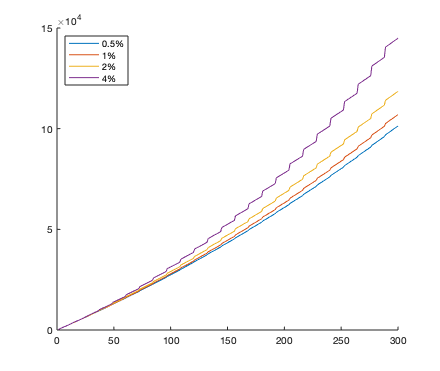
\includegraphics[width=0.45\textwidth]{res/op2.png}
\caption{Simulatie van spaarrekeningen met verschillende rentevoeten.}
\label{fig:op2}
\end{figure}

%%%
%%%
%%%

\fakesubsection{Opdracht 3}

Het bestand wordt ingeladen.

\begin{lstlisting}
load('Funds.mat')
\end{lstlisting}

%%%
%%%
%%%

\fakesubsection{Opdracht 4}

Men kan de parameters berekenen door eerst $\sigma$ te bepalen op basis van de rendementen, het gemiddelde te berekenen van diezelfde rendementen en vervolgens $\mu$ daaruit te bepalen.\\
\par\noindent De bekomen parameters bedragen $\mu = 3.208565\times 10^{-3}, \sigma = 3.070426\times 10^{-2}$ (voor \texttt{EUN5}) en $\mu = 7.857782\times 10^{-3}, \sigma = 3.277546\times 10^{-2}$ (voor \texttt{VWRL}).

\begin{lstlisting}
function [mu,sigma] = s0216676_estimateParameters(s)
    rendements = log(s(2:end) ./ s(1:end-1)); % Base doesn't matter
    sigma = std(rendements);
    mu = mean(rendements) + 0.5 * sigma^2;
end
\end{lstlisting}

%%%
%%%
%%%

\fakesubsection{Opdracht 5}

De implementatie maakt gebruik van een eenvoudige \mcode{for} loop.

\begin{lstlisting}
function [path] = s0216676_simulateFundPath(initialPrice, mu, sigma, months)
    alpha = mu - 0.5 * sigma^2;
    path = [initialPrice 2:months];
    for t = 2:months
        path(t) = path(t-1) * exp(alpha + sigma * randn);
    end
end
\end{lstlisting}

%%%
%%%
%%%

\fakesubsection{Opdracht 6}

In figuur \ref{fig:op6} worden de resulterende paden afgebeeld. Een aantal paden wijken af van de werkelijke koers afgebeeld in de opgave, maar de meesten komen realistisch over. De initi\"ele waarde bedraagt telkens 74.19 euro wat overeenstemt met de waarde in dollar op 26 november 2019.

\begin{figure}[h]
\centering
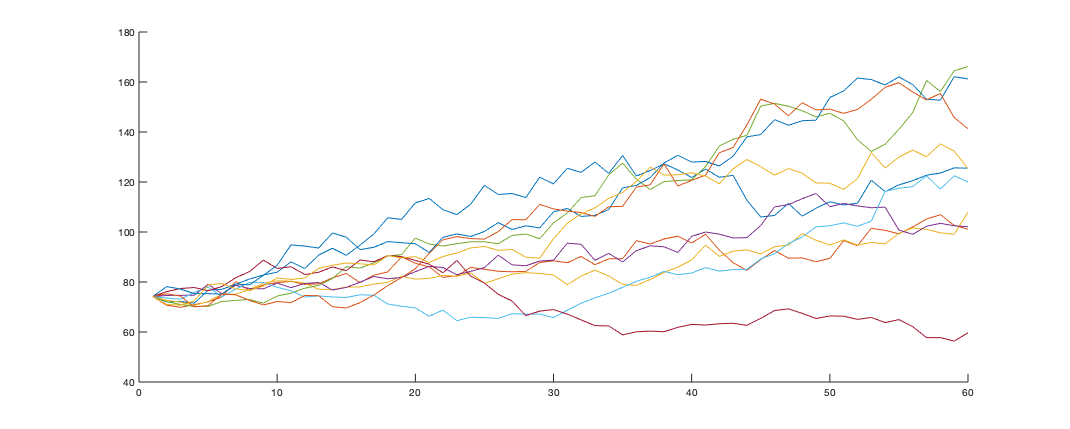
\includegraphics[width=\textwidth]{res/op6.png}
\caption{Simulatie van spaarrekeningen met verschillende rentevoeten.}
\label{fig:op6}
\end{figure}

\begin{lstlisting}
figure; hold all;
for i = 1:10
    plot(s0216676_simulateFundPath(74.19, mu, sigma, 60)); % Converted to euros (26/11/2019)
end
\end{lstlisting}

%%%
%%%
%%%

\fakesubsection{Opdracht 7}

aa

\begin{lstlisting}

\end{lstlisting}




